% Thrust 1, second round: answers to the notes of the last meeting.
% Compile on Overleaf with pdfLaTeX. Figures come from figures4papers/figure_Thrust1UQ/plot_feedback.py;
% Final figures (fig_fn_*): python plot_final.py, drawn at slide size (14 cm wide, 6-7.5 pt text).
% Older figures: python plot_feedback.py round2 (reads uq/director_comparison/summary.json and */conformal_ood.json).
\documentclass[aspectratio=169,11pt]{beamer}
\usetheme[progressbar=frametitle,numbering=fraction,block=fill]{metropolis}

\usepackage[utf8]{inputenc}
\usepackage{amsmath,amssymb,bm}
\usepackage{graphicx}
\usepackage{booktabs,array}
\usepackage{xcolor}
\graphicspath{{figures/}}

\definecolor{ourblue}{HTML}{0F4D92}
\definecolor{thrustred}{HTML}{B64342}
\definecolor{inkgrey}{HTML}{767676}
\setbeamercolor{alerted text}{fg=thrustred}
\setbeamercolor{block title}{bg=ourblue!15,fg=black}
\setbeamercolor{block body}{bg=ourblue!4}

\newcommand{\E}{\mathbb{E}}
\newcommand{\x}{\bm{x}}
\newcommand{\source}[1]{\par\vfill{\scriptsize\color{inkgrey}#1}}
\newcommand{\pending}{\textcolor{inkgrey}{pending}}

\title{Uncertainty in Compiled Feature Flows: Round 2}
\subtitle{What we did on the notes of the last meeting}
\author{Your Name}
\institute{Progress report, meeting with Prof.~Nghia}
\date{\today}

\begin{document}

\maketitle

% ============================================================
\begin{frame}{The notes of the last meeting, and what we did}
  \footnotesize
  \begin{tabular}{@{}p{0.27\linewidth}p{0.55\linewidth}p{0.12\linewidth}@{}}
    \toprule
    Note & This round & Status\\
    \midrule
    NLP data; fine-tune the model & Qwen2.5-0.5B fully fine-tuned on CoLA, SST-2, IMDB with DIRECTOR's splits, 5 seeds each & done\\
    Calibrate empirically on held-out data & Every threshold, temperature and certificate comes from held-out splits; the FM's training data never calibrates & done\\
    Conformal $\to$ guarantee on the true label $\to$ input guarantee & Group-conditional (Mondrian) guarantees, Theorems A--F; exact per-input validity is impossible & done\\
    Learn only the parameters and the threshold & Distance learned on A1, threshold level conformal on A2, aggressiveness certified on calB; ID likelihood cannot learn the threshold & done\\
    Input $\to$ conformal $\to$ threshold $\to$ input-specific uncertainty & Per-input jump rate from a group conformal p-value & done\\
    Use calibration to learn threshold and distance & As above, each on its own split & done\\
    Next: performance on ImageNet & Like-for-like evaluation in DIRECTOR's metrics (ImageNet, CIFAR, NLP); compiled on all 1.28M images: last 4 blocks $80.7\%$ agreement, all 12 blocks $45.3\%$ & done\\
    \bottomrule
  \end{tabular}
\end{frame}

% ============================================================
\section{Calibration protocol}

\begin{frame}{Every learned quantity has its own held-out split}
  \small
  \begin{tabular}{@{}llp{0.52\linewidth}@{}}
    \toprule
    Data & Used for & Why it must be separate\\
    \midrule
    FM training set (pool) & class means, covariance, regeneration targets & only defines the scaffold; never calibrates\\
    A1 (half of calA) & learn the distance $s_\theta$, temperature $T$ & must not see the calibration points\\
    A2 (other half) & conformal thresholds / p-values of $s_\theta$ & exchangeable with test given $\theta$ (Thm A)\\
    calB & Learn-then-Test certificate, choice of $(\alpha,\kappa,\tau)$ & candidates fixed by A1, A2 before calB is seen (Thm F)\\
    calC ($\tfrac14$ of test) & conformal label sets on $q$ & $q$ depends on A1, A2 and calB (Thm D)\\
    rest of test, shift, OOD & report only & \\
    \bottomrule
  \end{tabular}
  \par\medskip
  ImageNet: 2.5k / 2.5k / 5k / 10k / 30k from the 50k validation images. CIFAR: calA and calB come from the training split (2.5k each), so exchangeability with the official test set is only approximate. NLP: the held-out sets of DIRECTOR's splits (A1 / A2 / calB: CoLA 227 / 227 / 454, IMDB 1,250 / 1,250 / 2,500, SST-2 218 / 218 / 436).
\end{frame}

% ============================================================
\begin{frame}{Thresholds fitted on the FM's training features exceed their level}
  \centering
  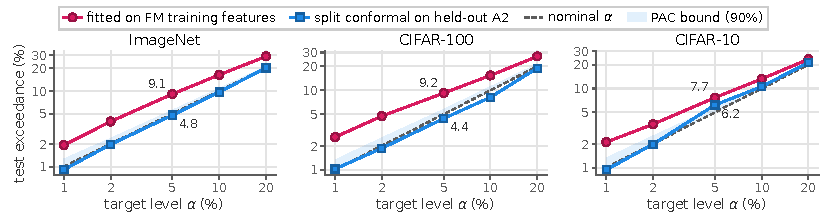
\includegraphics[width=\linewidth]{fig_fn_train_vs_heldout.pdf}
  \par\smallskip\raggedright\small
  \begin{itemize}
    \item Same learned score, threshold at the $(1-\alpha)$ quantile of the training features versus split conformal on A2. At $\alpha=5\%$, the training-feature threshold is exceeded by $9.1\%$ of ImageNet and $9.2\%$ of CIFAR-100 test inputs; held-out gives $4.8\%$ and $4.4\%$.
    \item The FM has fitted its training set, so its training features sit closer to the class means than new inputs. Held-out calibration is what makes $\alpha$ mean something.
  \end{itemize}
\end{frame}

% ============================================================
\section{Method: input $\to$ conformal $\to$ threshold $\to$ input-specific rate}

\begin{frame}{The method at a glance}
  \centering
  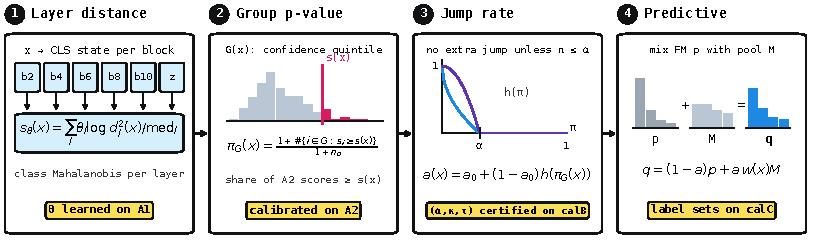
\includegraphics[width=\linewidth]{fig_fn_pipeline_method.pdf}
  \par\medskip\raggedright\small
  \begin{itemize}
    \item Each learned quantity has its own held-out split (yellow tags): the distance on A1, its level on A2, the aggressiveness on calB, the label sets on calC.
    \item One regeneration decision after the last layer, with a rate that depends on the whole path; an input pays nothing unless its group p-value is below $\alpha$.
  \end{itemize}
\end{frame}

% ============================================================
\begin{frame}{From input to input-specific uncertainty in four steps}
  \small
  \begin{enumerate}
    \item \textbf{Distance.} Layer distances $d_l^2(\x)$ (class Mahalanobis at the CLS after blocks $2,4,\dots,10$ and $z$), combined into a learned score
      \[ s_\theta(\x)=\textstyle\sum_l \theta_l \log\big(d_l^2(\x)/\mathrm{med}_l\big),\qquad \theta\in\Delta . \]
    \item \textbf{Conformal p-value} within the group $G(\x)$ (FM confidence quintile), on A2:
      \[ \pi_G(\x)=\frac{1+\#\{i\in A2:\ G_i=G(\x),\ s_i\ge s(\x)\}}{1+\#\{i\in A2:\ G_i=G(\x)\}} . \]
    \item \textbf{Input-specific jump rate}, zero cost unless $\x$ is in the top $\alpha$ of its group:
      \[ a(\x)=a_0+(1-a_0)\,h(\pi_G(\x)),\qquad h(u)=1-\big(\min(u/\alpha,1)\big)^{\kappa}. \]
    \item \textbf{Closed-form predictive} (path scaffold, every layer marginal preserved):
      \[ q(\cdot\mid\x)=(1-a(\x))\,p(\cdot\mid\x)+a(\x)\,w(\x)M,\quad M_c=\frac{\sum_j a_j w_c(\x_j)\,p(\cdot\mid\x_j)}{\sum_j a_j w_c(\x_j)}. \]
  \end{enumerate}
  \source{One regeneration decision after the last layer, with a rate that depends on the whole path: drawing a pool path with weight $a\,w_c$ keeps the joint law of all layer states. One score replaces $L$ thresholds, so the union bound $L\alpha$ becomes $\alpha$. Variant ``TS+scaffold'': $p$ replaced by the temperature-scaled FM, $T$ fitted on A1.}
\end{frame}

% ============================================================
\begin{frame}{The threshold cannot be learned from in-distribution likelihood}
  \begin{columns}[T,onlytextwidth]
    \column{0.50\textwidth}
    \small
    \textbf{Lemma.} If the FM is calibrated in distribution, $p(\cdot\mid\x)=P(Y\mid X=\x)$, then for any scaffold
    \[ \E\,[-\log q(Y\mid X)]\ \ge\ \E\,[-\log p(Y\mid X)] \]
    (Gibbs' inequality, pointwise in $\x$). The NLL-optimal threshold is $b=+\infty$: no jump.
    \medskip

    \textbf{Observed}, learning $(\theta,b,\beta,a_0,\tau)$ jointly by A1 NLL: on CIFAR-100 and ImageNet the learned $b$ is above every A1 score (no jump). On CoLA, where the FM is overconfident, the fit jumps on $99.8\%$ of inputs: a global softening, i.e.\ a worse temperature scaling.
    \column{0.46\textwidth}
    \small
    \textbf{So each part of $b$ has its own rule:}
    \begin{itemize}
      \item \emph{where to measure}: the distance $\theta$ is \textbf{learned} on A1, by non-negative logistic regression of the FM's errors on the layer distances;
      \item \emph{what $b$ means}: its level $\alpha$ is \textbf{calibrated} on A2 (split conformal, per group);
      \item \emph{how aggressive}: $(\alpha,\kappa,\tau)$ is \textbf{certified} on calB, taking the most sensitive candidate whose ID cost is proven small.
    \end{itemize}
  \end{columns}
\end{frame}

% ============================================================
\begin{frame}{The learned distance finds near-OOD inputs, but not errors as well as the softmax}
  \small
  \centering
  \begin{tabular}{@{}lcccccc@{}}
    \toprule
    & \multicolumn{2}{c}{Error AUROC (test)} & \multicolumn{2}{c}{Near OOD} & \multicolumn{2}{c}{Far OOD (Textures)}\\
    \cmidrule(lr){2-3}\cmidrule(lr){4-5}\cmidrule(lr){6-7}
    Score & CIFAR-100 & ImageNet & C100 vs C10 & ImageNet-O & CIFAR-100 & ImageNet\\
    \midrule
    uniform $\theta$ (multi-layer) & 0.648 & 0.614 & 0.702 & 0.891 & 0.986 & \textbf{0.970}\\
    learned by A1 NLL & 0.597 & 0.579 & 0.557 & 0.840 & 0.983 & 0.935\\
    learned on A1 errors & 0.825 & 0.761 & \textbf{0.961} & \textbf{0.925} & 0.983 & 0.898\\
    \midrule
    softmax (TS), $1-\max_y p_T$ & \textbf{0.923} & \textbf{0.874} & 0.909 & 0.847 & 0.955 & 0.858\\
    \bottomrule
  \end{tabular}
  \par\medskip\raggedright
  \begin{itemize}
    \item The error-trained weights put all mass on $z$ in every dataset; uniform weights keep the early layers that see textures and noise.
    \item For in-distribution errors the softmax is the better signal: errors sit near class boundaries, not far from the class means. The distance is an atypicality score.
  \end{itemize}
\end{frame}

% ============================================================
\section{Input-level guarantees}

\begin{frame}{What can be guaranteed about an individual input}
  \small
  \begin{itemize}
    \item \textbf{Not possible:} exact input-conditional validity, $P(Y\in C(X)\mid X=\x)\ge1-\alpha$ for every distribution and almost every $\x$, forces trivial sets at non-atomic $\x$ (Vovk, 2012; Lei and Wasserman, 2014; Foygel Barber et al., 2021).
    \item \textbf{Possible, from weakest to strongest:}
      \begin{enumerate}
        \item marginal: averaged over all inputs (our first version);
        \item group-conditional: for every group $G$ of inputs defined from $\x$ alone (Mondrian conformal);
        \item shift-conditional: for every reweighting of $P_X$ in a function class (Gibbs, Cherian and Cand\`es, 2023); groups are its indicator case;
        \item per-input and deterministic: argmax preservation, checked exactly for each $\x$.
      \end{enumerate}
    \item The price of finer groups is visible in the bounds: slack $1/(n_G+1)$ and larger thresholds, with $n_G$ the calibration points of the group. On CoLA ($n_G\approx45$) no group p-value can go below $\approx0.022$, so $\alpha=1\%$ is out of reach.
  \end{itemize}
\end{frame}

% ============================================================
\begin{frame}{Theorems A to C: thresholds, jump budget and flips per group}
  \small
  Exchangeable ID inputs; $s$ and $G$ fixed before A2 is seen; $n_k$ the A2 points in group $k$.
  \begin{block}{A. Group-conditional threshold}
    $\hat b_k=$ the $\lceil(n_k+1)(1-\alpha)\rceil$-th smallest A2 score of group $k$. Then $P\big(s(X)>\hat b_k\mid G(X)=k\big)\le\alpha$.
  \end{block}
  \begin{block}{B. Distribution-free jump budget}
    $P(\pi_k(X)\le t\mid G=k)\le t$, and $h$ is decreasing, so $\E[h(\pi_k)]=\int_0^1P(h(\pi_k)>v)\,dv\le\int_0^1h$. Hence
    \[ \E\big[\mathrm{TV}(q(\cdot\mid X),p(\cdot\mid X))\mid G=k\big]\le\E[a(X)\mid G=k]\le a_0+(1-a_0)\,\frac{\alpha\kappa}{\kappa+1}. \]
  \end{block}
  \begin{block}{C. Flips}
    If $\pi_k(\x)>\alpha$ then $a(\x)=a_0$; a flip needs $(1-a)\Delta\le a$. So $P(\text{flip}\mid G=k)\le\alpha+P\big(\Delta\le\frac{a_0}{1-a_0}\mid G=k\big)$, with $\Delta$ the FM top-2 margin.
  \end{block}
\end{frame}

% ============================================================
\begin{frame}{Theorems D to F: label sets, calibration-conditional and certified selection}
  \small
  \begin{block}{D. Group-conditional label sets on the scaffold}
    $C(\x)=\{y:1-q(y\mid\x)\le\hat t_{G(\x)}\}$, with $\hat t_k$ the conformal quantile on calC. Then $P(Y\in C(X)\mid G=k)\ge1-\alpha$.
  \end{block}
  \begin{block}{E. Calibration-conditional (PAC)}
    Given A2, the exceedance $P(s(X)>\hat b\mid A2)$ is $\mathrm{Beta}(n+1-l,\,l)$, $l=\lceil(n+1)(1-\alpha)\rceil$ (Vovk, 2012). With probability $\ge1-\delta$ over A2 it is below the $(1-\delta)$ Beta quantile.
  \end{block}
  \begin{block}{F. Learn-then-Test (Angelopoulos et al., 2021)}
    For each candidate $\lambda=(\alpha,\kappa,\tau)$, Hoeffding-Bentkus p-values for $H_\lambda: R_{\text{flip}}>1\%$ or $R_{\text{jump}}>5\%$ on calB. The certified set $\hat\Lambda$ satisfies
    \[ P\big(\exists\lambda\in\hat\Lambda:\ R_{\text{flip}}(\lambda)>1\%\ \text{or}\ R_{\text{jump}}(\lambda)>5\%\big)\le\delta=0.1, \]
    so any rule that picks inside $\hat\Lambda$ (lowest NLL, most sensitive) keeps the guarantee.
  \end{block}
  \source{Bonferroni over 40 candidates certifies nothing on CoLA (calB = 454: zero flips give $p=0.99^{454}=0.010>0.00125$). Fixed-sequence testing along each $\tau$ chain, ordered by the budget bound, is also valid and certifies 22 of 40.}
\end{frame}

% ============================================================
\begin{frame}{A marginal threshold hides a 3 to $6\times$ violation on uncertain inputs}
  \centering
  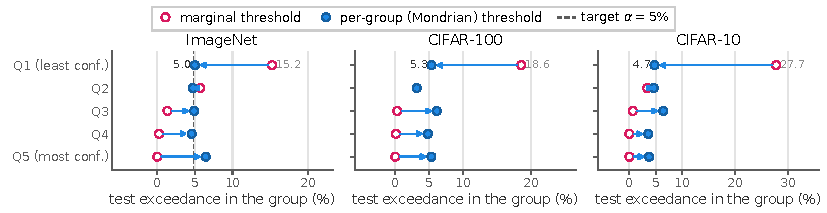
\includegraphics[width=\linewidth]{fig_fn_group_exceedance.pdf}
  \par\smallskip\raggedright\small
  \begin{itemize}
    \item Learned (error) distance, $\alpha=5\%$. Marginal: $5\%$ on average, but $15.2\%$ (ImageNet), $18.6\%$ (CIFAR-100) and $27.7\%$ (CIFAR-10) in the least confident quintile (open circles). Per group (filled): $4.6$ to $6.5\%$ on ImageNet.
    \item CIFAR's held-out split comes from the training set (accuracy $99.0\%$ versus $98.8\%$ on the official test set), so exchangeability is only approximate there; ImageNet's splits are exchangeable by construction.
  \end{itemize}
\end{frame}

% ============================================================
\begin{frame}{Label sets: per-group calibration repairs the worst group}
  \centering
  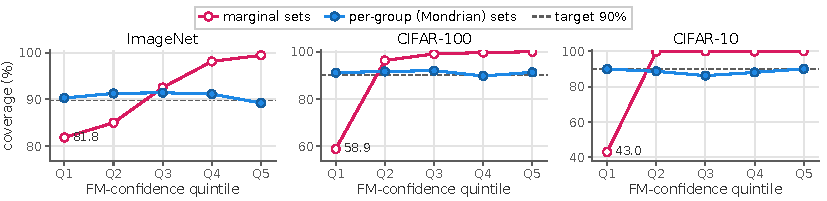
\includegraphics[width=\linewidth]{fig_fn_label_sets.pdf}
  \par\smallskip\raggedright\small
  \begin{itemize}
    \item Target $90\%$. Marginal sets cover the least confident quintile at $81.8\%$ (ImageNet), $58.9\%$ (CIFAR-100) and $43.0\%$ (CIFAR-10). Per-group sets: $90.3\%$, $91.1\%$, $89.9\%$.
    \item The gain comes from per-group calibration, not from the scaffold: Mondrian sets on the FM itself have the same coverage and size (ImageNet, $90\%$: $0.907$ / $2.00$ labels versus $0.905$ / $1.99$).
  \end{itemize}
\end{frame}

% ============================================================
\begin{frame}{The jump budget holds on every candidate; LTT keeps the certified ones}
  \centering
  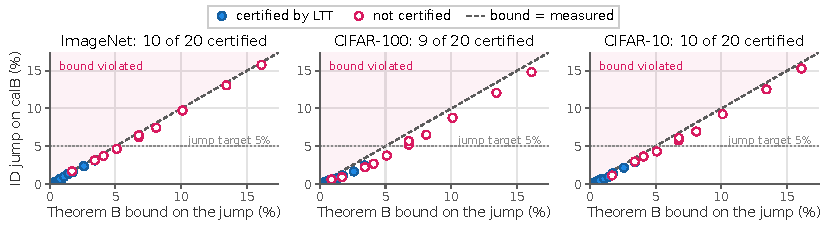
\includegraphics[width=\linewidth]{fig_fn_ltt_budget.pdf}
  \par\smallskip\raggedright\small
  Population target ($\tau=\infty$), 20 candidates $(\alpha,\kappa)$ per dataset. The measured ID jump mass never exceeds the bound of Theorem B (no point in the shaded region). Filled: certified by LTT for flip $\le1\%$ and jump $\le5\%$ at $\delta=0.1$ (9 or 10 of these 20; 21 to 23 of 40 when $\tau=1$ is included).
\end{frame}

% ============================================================
\section{Performance, like for like in DIRECTOR's metrics}

\begin{frame}{Evaluation protocol}
  \small
  \begin{itemize}
    \item \textbf{Same backbone, splits and metrics for every row.} DIRECTOR's metrics and units: ACC / MCC, AURC, failure AUROC, FPR95, ECE (\%), NLL ($\times10$), Brier (\%); on the in-distribution test split, on the shift sets, and OOD detection (AUROC / AUPR by MSP and entropy).
    \item \textbf{Rows.} FM; TS with $T$ fitted on the whole held-out set (the most favourable choice for the baseline); test-time dropout (MCD); deep ensemble (5 seeds for NLP, 3 checkpoints for ImageNet; $5\times$ / $3\times$ cost, shown but not ranked); certified scaffold on the FM and on the TS predictive, $\tau=1$ and $\tau=\infty$.
    \item \textbf{Fixed in advance.} Scaffold rows use the uniform distance and the most sensitive LTT-certified candidate; no row is picked after looking at test, shift or OOD data.
    \item \textbf{Seeds.} NLP: mean $\pm$ s.e. over 5 fine-tuning seeds. Vision: one fine-tuned checkpoint, so no error bars.
  \end{itemize}
  \source{Code: uq/imagenet\_ladder/director\_metrics.py, director\_eval.py, run\_director.sh. Tables: uq/director\_comparison/tables.md.}
\end{frame}

% ============================================================
\begin{frame}{CoLA, IMDB and SST-2, Qwen2.5-0.5B: the TS+scaffold ties temperature scaling}
  \centering
  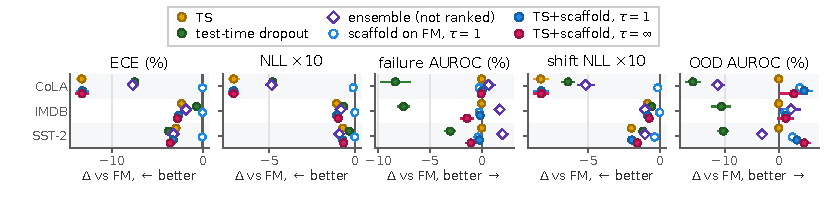
\includegraphics[width=\linewidth]{fig_fn_nlp_delta.pdf}
  \par\smallskip\raggedright\scriptsize
  \begin{itemize}
    \item \textbf{CoLA:} ECE $4.69\pm0.44$ (TS) vs $4.77\pm0.57$ (TS+scaffold), NLL$\times10$ $4.48$ vs $4.47$, failure AUROC $75.6$ vs $75.7$: a tie. \textbf{IMDB:} ECE $1.69\pm0.09$ vs $1.39\pm0.14$, NLL$\times10$ $1.41$ for both, failure AUROC $89.0$ vs $88.8$. \textbf{SST-2:} ECE $2.84\pm0.18$ vs $2.53\pm0.28$, NLL$\times10$ $1.98$ vs $1.97$, Brier $11.31$ vs $11.39$, failure AUROC $88.0$ vs $87.8$: at most a small ECE gain.
    \item On the raw FM the scaffold barely moves calibration, since the FM's problem (overconfidence everywhere, $T\approx4.7$ on CoLA, $2.4$ on IMDB, $2.0$ on SST-2) is global. Test-time dropout lowers failure AUROC on all three tasks ($75.6\to67.3$, $89.0\to81.4$, $88.0\to85.0$).
    \item \textbf{Shift} (SST-2 $\to$ IMDB, Yelp): TS+scaffold has the lowest ECE ($4.07\pm0.31$ vs TS $5.84\pm0.37$) at equal NLL$\times10$ ($4.00$ vs $3.98$). \textbf{OOD} (entropy AUROC): CoLA $73.4\to78.1$; SST-2 $84.5\to87.8$; IMDB $92.2\to93.5$, within the error.
  \end{itemize}
  \source{Figure: change against the FM, mean $\pm$ s.e.\ of the per-seed differences (5 seeds); left of 0 is better for ECE and NLL. IMDB's and SST-2's shift column is accuracy, CoLA's is MCC. Not comparable with DIRECTOR's Table 1 (CoLA MCC $\approx50$ vs $\approx30$, IMDB accuracy $95.3$ vs $85.6$): pre-trained Qwen versus 5-layer transformers trained from scratch. SST-2 is comparable with their Table 7 (Qwen2.5): see ``Relation to DIRECTOR's reported results''.}
\end{frame}

% ============================================================
\begin{frame}{Vision: ties in distribution, and the certificate does not cover shift}
  \centering
  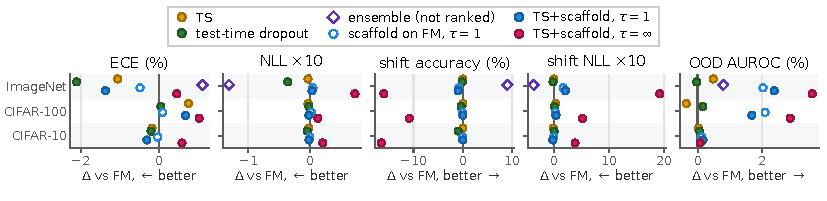
\includegraphics[width=\linewidth]{fig_fn_vision_delta.pdf}
  \par\smallskip\raggedright\small
  \begin{itemize}
    \item In distribution the scaffold stays within a few tenths of TS (accuracy kept, as certified); test-time dropout is the best single model on ImageNet.
    \item \alert{The LTT certificate is an ID statement.} Under shift many inputs jump: with $\tau=\infty$ accuracy falls $67.1\to51.0$ (ImageNet) and $75.9\to65.0$ (CIFAR-100); on ImageNet even $\tau=1$ raises shift NLL$\times10$ $14.0\to16.1$.
  \end{itemize}
  \source{Change against the FM; one fine-tuned checkpoint per dataset (no error bars). CIFAR-10: TS+scaffold ($\tau=1$) has the best shift calibration (CIFAR-10-C ECE $2.71$ vs TS $3.68$).}
\end{frame}

% ============================================================
\begin{frame}{OOD detection is where the scaffold helps}
  \centering
  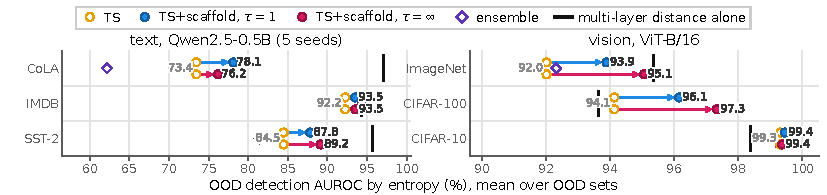
\includegraphics[width=\linewidth]{fig_fn_ood_compare.pdf}
  \par\medskip\raggedright\small
  \begin{itemize}
    \item The TS+scaffold improves OOD detection on CoLA ($73\to78$), SST-2 ($84.5\to87.8$--$89.2$), ImageNet ($92\to95$) and CIFAR-100 ($94\to97$). On IMDB the gain ($92\to93.5$) is within the error and the ensemble is higher ($94.5$).
    \item On CoLA, IMDB, SST-2 and ImageNet it stays below the distance score it is built on (black tick; SST-2: $95.7$): a two-class predictive is a narrow channel for atypicality. On CIFAR it exceeds it, because it keeps the softmax's near-OOD signal (CIFAR-10 vs CIFAR-100, where the multi-layer distance scores only $70$).
    \item NLP: AG News and 20 Newsgroups are still English text (for CoLA, its acceptability can be judged); only random-token sequences are clearly outside the task.
  \end{itemize}
\end{frame}

% ============================================================
\begin{frame}{Where the method stands: a structural ceiling}
  \small
  \begin{itemize}
    \item \textbf{Action.} Marginal preservation allows only one move: mix $p$ towards the pool predictive $M$. On a calibrated FM this can only raise ID NLL (Lemma); on an overconfident FM, one temperature fixes the global problem better.
    \item \textbf{Trigger.} The distance measures atypicality, not risk of error: softmax error AUROC $0.874$ vs $0.761$ (ImageNet).
    \item \textbf{Channel.} Atypicality must pass through the entropy of $q$; the pool target is not maximally uncertain and conformal p-values saturate at $1/(n_G+1)$. Result: OOD AUROC of $q$ below the distance on CoLA and ImageNet; above it on CIFAR only through the softmax's near-OOD signal.
    \item \textbf{Shift.} The distance does not separate ``corrupted but still correct'' from ``outside the task'', so OOD gains cost shift NLL.
    \item \textbf{Guarantees.} Theorems B, C, F bound how far $q$ moves from $p$ (do-no-harm); D holds for any base predictive, including the FM.
  \end{itemize}
  \medskip
  \centering
  \begin{tabular}{@{}l@{}}
    \toprule
    Ceiling: ID calibration $\le$ TS, \ OOD detection $\approx$ the better of softmax and distance.\\
    \bottomrule
  \end{tabular}
\end{frame}

% ============================================================
\section{Option 1: TS for probabilities, a conformal flag for atypical inputs}

\begin{frame}{Option 1: separate the two outputs}
  \small
  \centering
  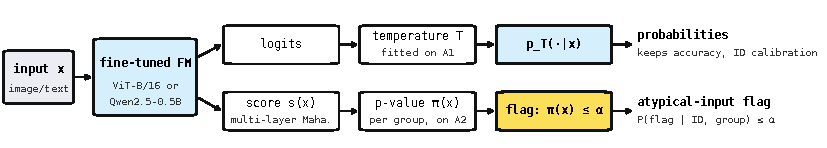
\includegraphics[width=\linewidth]{fig_fn_pipeline_option1.pdf}
  \raggedright
  \begin{block}{Guarantees (exchangeable ID inputs, score and groups fixed before A2)}
    \begin{itemize}
      \item ID false-alarm rate: $P(\text{flag}\mid\text{ID})\le\alpha$, and $\le\alpha$ in every group (Mondrian).
      \item PAC: with probability $\ge1-\delta$ over A2, the false-alarm rate is below the Beta quantile (Thm E).
      \item Batch: Benjamini--Hochberg on the conformal p-values controls the FDR of the flagged set, in expectation over A2 (Bates et al., 2023).
    \end{itemize}
  \end{block}
  \small
  Scores, fixed in advance and fitted without OOD data: $1-\max p_T$, entropy, energy, Mahalanobis at $z$, relative Mahalanobis at $z$, multi-layer Mahalanobis (uniform; primary) and learned on A1 errors.
  \source{Code: uq/imagenet\_ladder/conformal\_ood.py. Tables: uq/conformal\_ood/tables.md. Novelty is modest: conformal outlier testing and Mahalanobis scores exist; the contribution is the combination with TS, the per-group guarantee and the evaluation on DIRECTOR's benchmarks.}
\end{frame}

% ============================================================
\begin{frame}{The flag's guarantee holds, per group with Mondrian calibration}
  \centering
  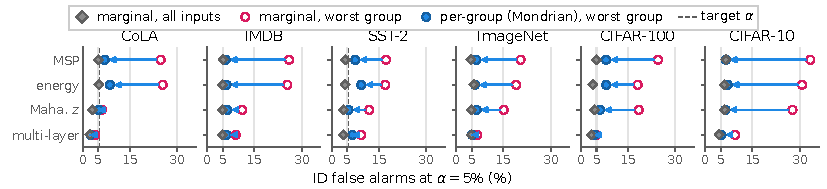
\includegraphics[width=\linewidth]{fig_fn_flag_validity.pdf}
  \par\medskip\raggedright\small
  \begin{itemize}
    \item Marginal false alarms (grey diamonds) stay at or close to $\alpha$ where splits are exchangeable (at most $5.6\%$ on CoLA, IMDB, SST-2, ImageNet, CIFAR-100); CIFAR-10 reaches $6.5\%$, its held-out data being drawn from the training split.
    \item A marginal flag concentrates its false alarms on the least confident inputs (worst group $17$--$33\%$ for softmax scores); Mondrian calibration brings the worst group to $2.5$--$9.4\%$ (the upper end on SST-2, with only $31$--$56$ A2 points per group).
    \item BH at $q=10\%$ controls the FDR in expectation over A2, not on each draw: the primary score stays at or below $9.5\%$ on every run, but MSP and $z$ reach $12$--$14\%$ on ImageNet's single split (with power $\le12\%$) and MSP $22\%$ on one IMDB seed.
  \end{itemize}
\end{frame}

% ============================================================
\begin{frame}{Its power depends on the score}
  \centering
  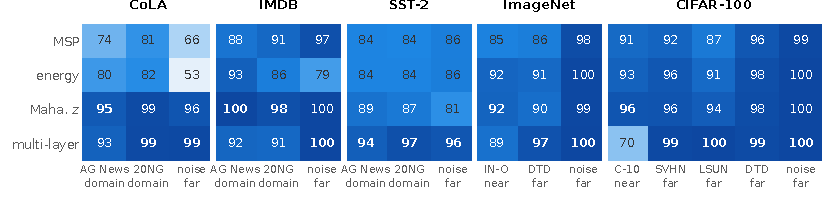
\includegraphics[width=\linewidth]{fig_fn_flag_power.pdf}
  \par\medskip\raggedright\small
  \begin{itemize}
    \item Distance scores beat the softmax scores that DIRECTOR's Table 5 uses, most clearly on Qwen (CoLA random tokens: $99.2$ vs $65.8$; IMDB, AG News: $99.7$ at $z$ vs $88.1$; SST-2, 20NG: $97.5$ multi-layer vs $83.8$).
    \item No single score wins both near OOD (Mahalanobis at $z$: CIFAR-10 vs CIFAR-100 $96.1$, ImageNet-O $92.5$) and far OOD (multi-layer: Textures $97.0$ on ImageNet). The primary score was fixed in advance and loses near OOD on CIFAR-100 ($70.2$); at $\alpha=5\%$ on IMDB it flags $35$--$43\%$ of out-of-domain text, against $89$--$100\%$ at $z$.
  \end{itemize}
  \source{Detection AUROC (\%), mean over seeds; bold: best score per OOD set. IN-O: ImageNet-O; DTD: Textures; C-10: CIFAR-10. CoLA: AG News and 20NG are out of domain but within the task. Relative Mahalanobis at $z$ (Ren et al., 2021), also fixed in advance, ranks the OOD sets of CoLA and IMDB below the in-distribution test set (AUROC under $6\%$); not shown.}
\end{frame}

% ============================================================
\begin{frame}{Two flags answer two different questions}
  \centering
  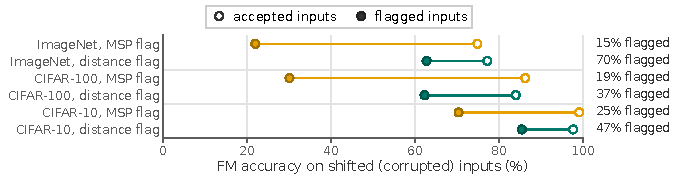
\includegraphics[width=0.82\linewidth]{fig_fn_flag_shift.pdf}
  \par\medskip\raggedright\small
  \begin{itemize}
    \item The softmax flag catches inputs the model will get wrong (flagged accuracy $30\%$ on CIFAR-100-C, $22\%$ on ImageNet): selective prediction. The distance flag catches inputs that look different, including corrupted images the FM still classifies correctly ($70\%$ of ImageNet's corrupted images flagged).
    \item \textbf{Next, at no cost to the guarantee:} flag when $\min(\pi_z,\pi_{\text{multi}})\le\alpha/2$ (Bonferroni). The false-alarm rate stays $\le\alpha$ without OOD data, and the flag should inherit near-OOD power from $z$ and far-OOD power from the multi-layer score.
  \end{itemize}
  \source{$\alpha=5\%$, marginal calibration; FM accuracy on accepted (open) and flagged (filled) shifted inputs.}
\end{frame}

% ============================================================
\section{DIRECTOR's benchmarks}

\begin{frame}{The NLP ladder follows DIRECTOR's text benchmarks}
  \small
  \begin{itemize}
    \item \textbf{Backbone.} Qwen2.5-0.5B (24 blocks, $d=896$), the model DIRECTOR reconfigures in App.~A.6.1, with a linear head on the last token. Full fine-tuning, 5 seeds per task; the 5 seeds also form a deep ensemble.
    \item \textbf{IMDB:} 20k fine-tune / 5k held out / 25k test (DIRECTOR's split sizes). Shift: SST-2 test, Yelp.
    \item \textbf{CoLA:} 6,355 / 907 / 1,816 from in-domain train + dev, as in DIRECTOR; shift: CoLA out-of-domain dev (516), their ``CoLA OOD''. Metric: MCC.
    \item \textbf{SST-2:} GLUE train phrases; held out: GLUE dev (872); test: SST-2 test sentences (1,821), disjoint from training sentences. Shift: IMDB, Yelp. All sets end with GLUE's trailing space token, because the head reads the last token.
    \item \textbf{OOD for every task:} AG News, 20 Newsgroups, random-token sequences.
  \end{itemize}
  \source{Code: uq/nlp\_ladder (nlp\_prepare.py, run\_nlp.sh). Results: mean $\pm$ s.e. over 5 seeds, as in DIRECTOR's tables.}
\end{frame}

% ============================================================
\begin{frame}{Relation to DIRECTOR's reported results}
  \small
  \begin{itemize}
    \item \textbf{Main axis (ID calibration).} DIRECTOR improves on TS for its small backbones (Tables 2, 10), and adds 2--4 accuracy points, which no post-hoc layer can. Our scaffold only ties TS. On pre-trained backbones, the comparable result is Table 7 (Qwen2.5, SST-2; next slide).
    \item \textbf{Secondary axes.} DIRECTOR's OOD table (Table 5) scores by MSP and entropy; on our backbones distance scores are much stronger, so the conformal flag of Option 1 could be added on top of a DIRECTOR model as well. The shift tables (3, 17, 18) do not include TS, which on CoLA-OOD is the best single model in our runs.
    \item \textbf{Reproduction.} Except for Table 7, backbones differ (pre-trained ViT-B/16 and Qwen versus small models trained from scratch). A reproduction of Tables 1--5 with the authors' code is running: 223 of 450 runs done; 21 CoLA / SVHN runs restarted after environment fixes; no tables yet.
  \end{itemize}
\end{frame}

% ============================================================
\begin{frame}{SST-2 with Qwen2.5-0.5B: temperature scaling beside DIRECTOR's Table 7}
  \centering
  \small
  \begin{tabular}{@{}lcccc@{}}
    \toprule
    SST-2, Qwen2.5-0.5B & ACC & ECE$\downarrow$ & NLL ($\times10$)$\downarrow$ & Brier$\downarrow$\\
    \midrule
    Qwen2.5 (DIRECTOR, Table 7) & 93.01 & 5.86 & 3.30 & 12.18\\
    DIRECTOR, last 3 blocks (Table 7) & 93.12 & 5.48 & 2.95 & 12.09\\
    \midrule
    Our FM (5 seeds) & 92.62 & 5.77 & 2.71 & 12.88\\
    \quad + TS ($T\approx2$) & 92.62 & 2.84 & 1.98 & \textbf{11.31}\\
    \quad + TS+scaffold, $\tau=1$ & 92.63 & \textbf{2.53} & \textbf{1.97} & 11.39\\
    \bottomrule
  \end{tabular}
  \par\medskip\raggedright\small
  \begin{itemize}
    \item Our fine-tune starts close to DIRECTOR's base model (accuracy $92.6$ vs $93.0$, ECE $5.77$ vs $5.86$).
    \item From there, TS alone lowers ECE by $2.9$ points and NLL$\times10$ by $0.73$; DIRECTOR's reconfiguration of the last 3 blocks lowers them by $0.38$ and $0.35$, and adds $0.1$ accuracy points.
    \item Table 7 has no TS row, so whether DIRECTOR adds to TS on Qwen is open; TS on top of the DIRECTOR model would settle it.
  \end{itemize}
  \source{Ours: mean over 5 fine-tuning seeds (s.e.\ of ECE $0.18$--$0.28$), test = SST-2 test sentences (1,821); TS row: $T$ on the whole held-out set, TS+scaffold: $T$ on A1. DIRECTOR's numbers as reported in its Table 7; separate fine-tunes, so the comparison is of the size of each step, not of the end points.}
\end{frame}

% ============================================================
\section{Full ImageNet-1k compilation}

\begin{frame}{Full-data compilation: the last 4 blocks reach 80.7\% agreement}
  \centering
  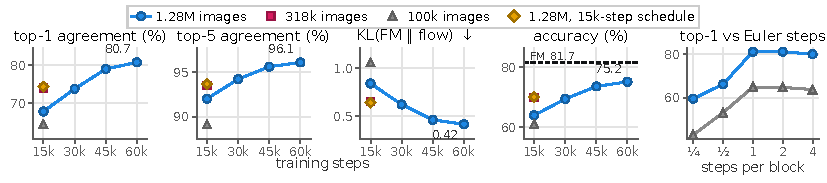
\includegraphics[width=\linewidth]{fig_fn_full_compile.pdf}
  \par\smallskip\raggedright\footnotesize
  \begin{itemize}
    \item \textbf{Result} (10k test images; 1.28M images, 60k steps): top-1 agreement $80.7\%$, top-5 $96.1\%$, KL $0.42$, accuracy $75.2$. The 318k-image arm: $74.0\%$, $93.5\%$, $0.66$, $70.0$. A clear gain, but the flow still changes about a fifth of the predictions and stays $6.5$ accuracy points below the FM (dashed).
    \item \textbf{The gain comes from steps, not data.} A 15k-step arm on all 1.28M images, with its own annealed schedule (amber diamond), matches the 318k arm: $74.3\%$ vs $74.0\%$ agreement, accuracy $70.1$ vs $70.0$. At 36 samples per step, 15k steps see $0.54$M samples, so neither arm is data-limited yet. Open: the 318k arm at 60k steps ($\approx7$ epochs).
    \item \textbf{Nearly step-stable from one Euler step per block on:} $81.0$, $81.0$, $79.9\%$ (KL $0.40$, $0.42$, $0.49$) at $1$, $2$, $4$ steps per block; below one step ($\tfrac12$: $66.1\%$) a step crosses a block boundary, where the teacher's velocity jumps. The 100k arm behaves the same ($64.9$, $64.7$, $63.7\%$): data raised fidelity, not step stability.
    \item \textbf{All 12 blocks:} $45.3\%$ (next slide).
  \end{itemize}
  \source{Code: uq/imagenet\_ladder/run\_full.sh, run\_full\_match15k.sh.}
\end{frame}

% ============================================================
\begin{frame}{Uncertainty on the full-data flow: still below the FM}
  \small
  \centering
  \begin{tabular}{@{}lccccc@{}}
    \toprule
    ImageNet, last 4 blocks compiled & ACC & NLL$\downarrow$ & ECE (\%)$\downarrow$ & Shift NLL$\downarrow$ & OOD AUROC\\
    \midrule
    FM (no compilation) & \textbf{81.68} & \textbf{0.694} & 4.00 & \textbf{1.401} & \textbf{0.915}\\
    \midrule
    Flow & 75.19 & 0.950 & 2.17 & 1.743 & 0.842\\
    Flow + TS & 75.19 & 0.950 & \textbf{1.66} & 1.747 & 0.846\\
    Flow + partitioned regeneration & 75.16 & 0.949 & 2.04 & 1.743 & 0.847\\
    Flow + certified scaffold, $\tau=1$ & 75.12 & 0.959 & 1.84 & 2.010 & 0.877\\
    Flow + certified scaffold, $\tau=\infty$ & 75.15 & 0.991 & 2.81 & 2.554 & 0.909\\
    \bottomrule
  \end{tabular}
  \par\medskip\raggedright
  \begin{itemize}
    \item The scaffold brings OOD detection on the flow close to the FM ($0.842\to0.909$ vs $0.915$), at the same price as on the FM: shift NLL rises from $1.74$ to $2.55$.
    \item The flow's ECE is lower than the FM's, yet its NLL is worse: the lost accuracy dominates. Temperature scaling does little here ($T\approx1$).
  \end{itemize}
  \source{Uniform distance, most sensitive LTT-certified candidate (Bonferroni); flips $\le0.6\%$. One compiled field, no error bars.}
\end{frame}

% ============================================================
\begin{frame}{All 12 blocks on all images: 45\% agreement, far from the FM}
  \centering
  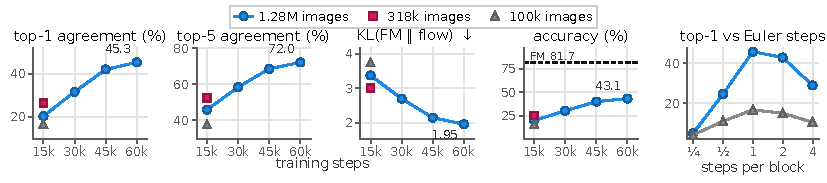
\includegraphics[width=\linewidth]{fig_fn_full_compile_all12.pdf}
  \par\smallskip\raggedright\footnotesize
  \begin{itemize}
    \item \textbf{Result} (1.28M images, 60k steps): top-1 agreement $45.3\%$, top-5 $72.0\%$, KL $1.95$, accuracy $43.1$ (FM $81.7$); the 318k arm at 15k steps: $26.4\%$, accuracy $25.2$. Snapshots at 15k/30k/45k/60k: $20.2$, $31.5$, $42.0$, $45.3\%$: still rising, but only $+3.3$ in the last 15k steps. (The 15k snapshot is below the 318k arm because its schedule has not annealed.)
    \item \textbf{Not a convergent ODE either:} $45.9$, $42.9$, $28.9\%$ at $1$, $2$, $4$ Euler steps per block ($-37\%$ at 4 steps, as in the 100k arm: $-38\%$); unlike the last 4 blocks, more steps make it worse.
  \end{itemize}
  \source{Code: uq/imagenet\_ladder/run\_full.sh all12. Agreement on 10k test images; FM accuracy dashed.}
\end{frame}

% ============================================================
\begin{frame}{Uncertainty on the 12-block flow: no scaffold can be certified}
  \small
  \centering
  \begin{tabular}{@{}lccccc@{}}
    \toprule
    ImageNet, all 12 blocks compiled & ACC & NLL$\downarrow$ & ECE (\%)$\downarrow$ & Shift NLL$\downarrow$ & OOD AUROC\\
    \midrule
    Flow & 43.17 & 2.503 & 3.04 & 4.792 & 0.546\\
    Flow + TS ($T=0.93$) & 43.17 & 2.496 & \textbf{1.07} & 4.876 & 0.524\\
    Flow + conformal scaffold (not certified) & 43.05 & 2.539 & 3.85 & 4.904 & \textbf{0.825}\\
    \bottomrule
  \end{tabular}
  \par\smallskip\raggedright
  \begin{itemize}
    \item The flow is more confident on random noise than on ImageNet images (noise AUROC $0.32$); the distance-driven scaffold repairs this ($0.99$), which lifts the mean OOD AUROC to $0.825$ (FM: $0.915$).
    \item LTT certifies none of the 40 candidates: the flow's margins are small, so every candidate flips $\ge0.78\%$ of calB, and the bound flip $\le1\%$ cannot be certified at $n=5$k under Bonferroni.
  \end{itemize}
  \source{Test split of the conformal protocol; scaffold row: uniform distance, marginal p-values, $\alpha=5\%$, $\kappa=1$, $\tau=\infty$.}
\end{frame}

% ============================================================
\section{Decisions for this meeting}

\begin{frame}{Four decisions}
  \small
  \begin{enumerate}
    \item \textbf{Marginal preservation.} Exact preservation holds for the pool (training) distribution only, and constrains the action to the pool target. Proposal: replace it by a certified approximate version that already follows from Theorem B,
      \[ \big\|\E_X q(\cdot\mid X)-\E_X p(\cdot\mid X)\big\|_{\mathrm{TV}}\le\E[a(X)]\le a_0+(1-a_0)\tfrac{\alpha\kappa}{\kappa+1}\quad\text{(ID, per group)}, \]
      which holds on the test distribution and leaves OOD inputs free. Acceptable for Thrust 1?
    \item \textbf{Positioning.} Option 1 (TS + conformal flag, honest and validated, modest novelty) versus continuing the scaffold (ties TS in distribution; OOD gains bounded by the better of softmax and distance).
    \item \textbf{Shift-aware variant.} A per-input temperature was considered; its ceiling is small even with an oracle (backup slide). Only a semantic OOD branch with a uniform target remains worth a pilot.
    \item \textbf{Full ImageNet.} What does Thrust 1 need from the compiled flow? Is $80.7\%$ agreement, $6.5$ accuracy points below the FM, acceptable for the last 4 blocks? All 12 blocks reach only $45\%$. Since steps, not data, drove the gain, is a longer run (or the 318k arm at 60k steps, to separate the two) worth the GPU time?
  \end{enumerate}
\end{frame}

% ============================================================
\begin{frame}{Summary}
  \footnotesize
  \begin{itemize}
    \item \textbf{Held out.} All thresholds, temperatures and certificates come from held-out data; training-feature thresholds overshoot their level ($9.1\%$ vs $5\%$ on ImageNet).
    \item \textbf{Threshold.} ID likelihood provably cannot learn it. The distance is learned, the level is conformal, the sensitivity is certified by Learn-then-Test (fixed-sequence for small calibration sets).
    \item \textbf{Input guarantees.} Per-group thresholds, jump budget, flip and label-set guarantees. Marginal calibration hides 3 to $6\times$ violations on uncertain inputs; per-group calibration removes them.
    \item \textbf{Performance, like for like.} In distribution the scaffold ties TS; it improves OOD detection (CoLA $73\to78$--$83$, SST-2 $84.5\to87.8$--$89.2$, ImageNet $92\to94$--$95$, CIFAR-100 $94\to96$--$97$; within the error on IMDB) but stays below the distance score on CoLA, IMDB, SST-2 and ImageNet, and the certificate does not cover shift. SST-2 (DIRECTOR's Table 7): TS alone lowers ECE $5.77\to2.84$, TS+scaffold $2.53$; DIRECTOR reports $5.86\to5.48$.
    \item \textbf{Option 1.} TS plus a conformal flag keeps every guarantee and the full detection power of the distance; the flag's validity holds where splits are exchangeable.
    \item \textbf{Compilation.} Last 4 blocks on all of ImageNet: agreement $74.0\to80.7\%$, accuracy $70.0\to75.2$ (FM $81.7$); the step-matched arm shows the gain comes from 4$\times$ more steps, not data. All 12 blocks: $26.4\to45.3\%$, accuracy $43.1$, no LTT-certified scaffold.
    \item \textbf{Running.} The reproduction of DIRECTOR's tables (223 of 450 runs).
  \end{itemize}
\end{frame}

% ============================================================
\appendix
\section*{Backup}

\begin{frame}{Backup: a per-input temperature has a small ceiling}
  \small
  \centering
  \begin{tabular}{@{}lcccc@{}}
    \toprule
    Shift NLL (natural units) & TS ($T_0$ on A1) & one oracle $T$ for all shift & oracle $T$ per corruption & per (corruption, severity)\\
    \midrule
    CIFAR-100-C & 1.051 & 1.012 & 1.006 & 1.001\\
    CIFAR-10-C & 0.290 & 0.276 & 0.272 & 0.269\\
    ImageNet, 4 corruptions & 1.397 & 1.397 & 1.395 & --\\
    \bottomrule
  \end{tabular}
  \par\medskip\raggedright
  \begin{itemize}
    \item Oracle temperatures fitted on the test shift data itself: an upper bound for any gate that only adjusts the temperature.
    \item At most $5\%$ NLL on CIFAR-100-C, most of it from one global shift temperature; nothing on ImageNet. On CIFAR the ID test set prefers $T_0$ while shift prefers a higher $T$ ($T_0=0.884$, oracle on ID test $0.922$), so the headroom is shift-specific, not an artifact of the split.
    \item Group-level oracle, not per-input; it bounds what a corruption-aware gate can gain.
  \end{itemize}
\end{frame}

\end{document}
